\documentclass{article}
\usepackage[utf8]{inputenc}
\usepackage{graphicx}
\usepackage{tikz}
\usepackage{float}
\usetikzlibrary{positioning,fit,calc,arrows.meta, shapes}
\graphicspath{ {images/} }

%Tot això hauria d'anar en un pkg, però no sé com és fa
\newcommand*{\assignatura}[1]{\gdef\1assignatura{#1}}
\newcommand*{\grup}[1]{\gdef\3grup{#1}}
\newcommand*{\professorat}[1]{\gdef\4professorat{#1}}
\renewcommand{\title}[1]{\gdef\5title{#1}}
\renewcommand{\author}[1]{\gdef\6author{#1}}
\renewcommand{\date}[1]{\gdef\7date{#1}}
\renewcommand{\maketitle}{ %fa el maketitle de nou
    \begin{titlepage}
        \raggedright{UNIVERSITAT DE LLEIDA \\
            Escola Politècnica Superior \\
            Grau en Enginyeria Informàtica\\
            \1assignatura\\}
            \vspace{5cm}
            \centering\huge{\5title \\}
            \vspace{3cm}
            \large{\6author} \\
            \normalsize{\3grup}
            \vfill
            Professorat : \4professorat \\
            Data : \7date
\end{titlepage}}
%Emplenar a partir d'aquí per a fer el títol : no se com es fa el package
%S'han de renombrar totes, inclús date, si un camp es deixa en blanc no apareix

\tikzset{
	%Style of nodes. Si poses aquí un estil es pot reutilitzar més facilment
	pag/.style = {circle, draw=black,
                           minimum width=0.75cm, font=\ttfamily,
                           text centered}
}
\renewcommand{\figurename}{Figura}
\title{Primera pràctica d'Inteligència Artificial}
\author{Joaquim Picó Mora}
\date{Divendres 15 de Novembre}
\assignatura{Inteligència Artificial}
\professorat{Carlos Ansotegui}
\grup{PraLab1}

%Comença el document
\begin{document}
\maketitle
\thispagestyle{empty}

\newpage
\pagenumbering{roman}
\tableofcontents
\newpage
\pagenumbering{arabic}

\section{Taula Evaluació Experimental}
\begin{figure}[h!]
	\centering
	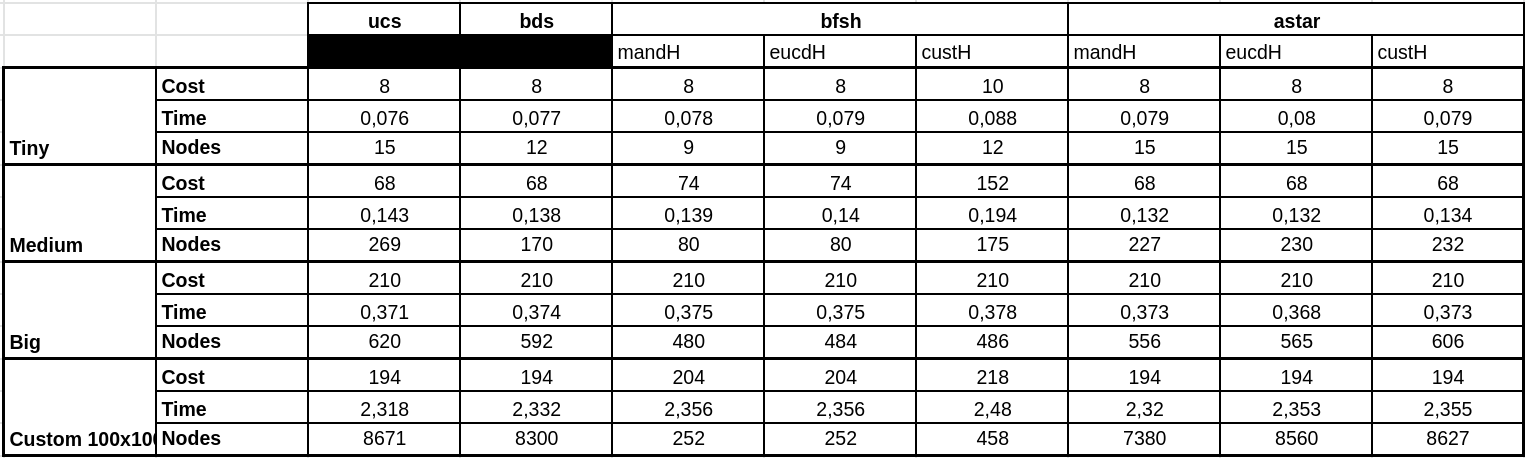
\includegraphics[width=0.7\textheight]{taula.png}
	\caption{Taula Evaluació Experimental.}
	\label{tee}
\end{figure}
\section{Algoritmes}
%
\subsection{Uniform Cost Search}
L'ucs és caracteritza per expandir sempre el node al que s'ha arribat amb el menor cost. Per a realitzar aixó he declarat la frontera com una cua per prioritat, fent així que cada cop que es tregui un element d'ella per a expandir-lo sigui el que te el cost més baix ja que la llista és trovarà ordenada per prioritat. 
\\\\
La principal característica d'aquest algorísme i que el fa diferir del Breath First Search és que si trobem un node n1 a la frontera que té un cost determinat, i un altre node n2 el qual ens porta al mateix estat que n1 i amb menor cost. Aleshores afegirem aquest segón node  a la frontera, i la mateixa cua per prioritat fara que n2 s'expandeixí abans que n1 ja que tindrà un cost menor i per tant una major prioritat.
\\\\
Aquest algoritme ens trobarà sempre el camí optim a la solució. En aquest cas però, al ser el cost lineal, l'espai d'estats finit, el factor de ramificació també finit i havent-hi solució, ens trobarà el camí optim, però executanse de forma identica a l'algoritme Breath First Search
\\\\
Podem veure en la Figura1 que l'ucs de tots els algoritmes proposats és el menys eficient en quant a espai. En canvis, el temps d'execució és molt proper al de tots els altres algorismes.
\subsection{Bidirectional Search}
S'ha decidit implementar mitjançant l'algoritme bfs desde dos punts diferents. Aquests punts són el punt d'inici i el punt d'arribada i cada un d'ells tindrà fronteres i llistes de nodes expandits diferents. 
\\\\
D'aquesta forma, cada cop que afegim un element a una de les dos fronteres, comprovarem que no es trovi a la llista de generats de l'altre.
\\\\
Quan es generen els nodes successors  que deriven del punt d'arribada, l'acció d'aquest s'haurà de canviar per la seva antagònica, fent d'aquesta forma que al concatenar els recorreguts el que en resulta sigui vàlid. Per tal de reaprofitar la mateixa funció s'ha decidit implementar-ho amb lambda functions.
\subsection{Greedy Best First Search}
En quant al bfsh, és una aplicació de l'ucs, pero en canvis d'expandir el node amb menor cost, expandeixen aquells amb l'heurística que més prometi. Per el demés, es segueix exactament el mateix patró de diseny que l'ucs.
\subsection{A*}
De misma forma que el bfsh el algoritmo A* es una derivación del ucs, pero ahora en canvio de expandir el nodo con la mejor heurística, expandirá el que su coste sumado a su heuristica sea el más pequeño.
De mateixa manera que el bfsh l'algoritme A* és una derivació del ucs, pero ara en canvi d'expandir el node amb la millor heurística, expandirá el que el seu cost sumat a la seva heurística sigui el mínim.
\\\\
Per assegurar la concistencia d'una heuristica donada l'admissibilitat, realitzem la funció getPriority la qual ens retornarà el maxim entre l'heurística més el cost entre pare i fill.
\\\\
\section{Heurístiques}
\subsection{Distancia de Manhattan}
Aquesta heurística consisteix en agafar la distancia total entre el node i la posició en la que volem arribar. Per a realitzar-ho sumem amb valor absolut la distancia entre node i goal en l'eix x més la distancia en l'eix y. 
\subsection{Distància d'Euclides}
La distància d'euclides consisteix a aplicar la regla de pitagores amb les distancies x i y calculades a l'apartat anterior per obtenir la distancia en línea recta en que es troba el node de la posició goal.
\subsection{Distancia xAxe}
Aquesta és l'heurítica que he proposat com alternativa. Consisteix en la distancia en l'eix de les x entre el node i la posició d'arribada.

\section{Anàlisis Evaluació Experimental}
Com podem veure, el que expandeix la menor quantitat de nodes i que per tant és el més eficient en termes d'espai és l'algoritme bfsh, aquest si existeix una solució ens la trobarà, pero no garantitza que aquesta sigui optimal. 
\\\\
Tots els altres algoritmes garanteixen que la solució que trobaràn serà l'optima, però es pot veure que el més eficient serà l'A* degut a que expandeix el menor nombre de nodes d'entre els algoritmes que garanteixen una solució optimal.\\
Seguidament a l'A* s'hi trova el bds, aquest expandeix menys nodes que l'ucs, aixó és degut a que expandeix des de dos punts diferents del mapa, i per tant l'amplada de l'expansió prop del punt de trobada serà menor que si ho fés només des d'un unic punt.
\\\\
Finalment trobel l'ucs com l'algorisme menys eficient dels optimals degut a que expandeix mes nodes que els altres dos algoritmes.
\\\\ 



\end{document}